\documentclass[9pt,twoside,lineno]{pnas-new}
% Use the lineno option to display guide line numbers if required.

\usepackage{bm}

\DeclareMathOperator\erf{\Phi}
\makeatletter
\newcommand{\ud}{\text{d}}
\let\originalleft\left
\let\originalright\right
\renewcommand{\left}{\mathopen{}\mathclose\bgroup\originalleft}
\renewcommand{\right}{\aftergroup\egroup\originalright}
\newcommand{\mat}[1]{\bm{#1}}

\templatetype{pnassupportinginfo}

\title{Your main manuscript title}
\author{Mikael Ohlsson, György Barabás, Max Lindmark, Michele Casini, Valerio Bartolino, Mattias Sköld \& Anna Eklöf}
\correspondingauthor{Corresponding author: Mikael Ohlsson.\\E-mail: mikael.ohlsson@liu.se}

\begin{document}

%% Comment out or remove this line before generating final copy for submission; this will also remove the warning re: "Consecutive odd pages found".
%\instructionspage  

\maketitle

%% Adds the main heading for the SI text. Comment out this line if you do not have any supporting information text.
\SItext


\bigskip

\section*{Details of the eco-evolutionary model} \label{sec:si_ecoevo}

\subsection*{Trait space and the per capita growth rates}

The model tracks the population density and body size distribution of two species through time. Here we focus on cod and flounder as the two species. We assume that the body size $z$ of an individual and the average size of its resources are sufficiently tightly correlated that $z$ need not refer to the actual body size, but instead to the mean body size of its prey \citep{Rossberg2013, Schneideretal2016}. Thus, we define $z = \log(B/B_0)$, where $B$ is the average resource size (assumed to be in a quasi-one-to-one relationship with the individual's size) and $B_0$ is a reference size which can be chosen without loss of generality. Here we set it to be the mean size of the flounder's prey. This choice means that $z = 0$ now corresponds to the point at which the mean prey size of cod and flounder coincide.

We make the important assumption that flounder body sizes do not evolve---this implies that $B_0$ is constant in the model. To describe the interactions between the two species, we assume that they compete for shared resources. Empirically, it is known that the diets of cod and flounder do overlap, but not completely. To account for the general possibility of incomplete overlap, we model resource consumption in a potentially high-dimensional trait space, the first of which is the body size $z$. The other traits (which may include preferred depth in the water, swimming speed, coloration, etc.) contribute to resource utilization, but are not under evolutionary influence: since the main driver of trait change is fishing pressure which primarily selects for size, we ignore selection on the other traits.

The ensemble of traits can be denoted with the vector $\mat{x}$, the first component of which is the body size $z$ by convention. Our goal is to derive a form for the per capita growth rate $r(\mat{x})$ of individuals with phenotype $\mat{x}$. The processes determining this growth rate are (1) growth due to consumption of resources, (2) natural mortality, (3) mortality due to size-dependent fishing pressure, (4) mortality from oxygen-deprived regions which affect bigger individuals more due to different food-seeking behaviour, and (5) competition from individuals with trait vector $\mat{x}'$ (irrespective of which species that phenotype belongs to). We can write this as follows:
\begin{equation}
  \label{eq-r}
  r(\mat{x})
  = \int u(\mat{x}, \mat{y}) R(\mat{y}) \,\ud\mat{y}
  - m(z)
  - f(z)
  - H(z),
\end{equation}
where the first term describes growth on (as well as competition for) shared resources, the second term $m(z)$ is natural mortality, the third $f(z)$ is mortality due to fishing, and the fourth $H(z)$ is mortality due to hypoxia. In the first term, $R(\mat{y})$ is the availability of resources of type $\mat{y}$, $u(\mat{x}, \mat{y})$ is the utilization of resource type $\mat{y}$ by an individual of phenotype $\mat{x}$, and the integration is understood to apply separately for each component of $\mat{y}$.

In turn, resource availability is given as the maximum (saturation) resource levels, minus what is currently being consumed by the cod and flounder populations. We make the assumption of time scale separation, with the resource dynamics being faster than the consumer dynamics \cite{MacArthur1970, Pastore2021, Barabasetal2022}. We then have
\begin{equation}
  \label{eq-R}
  R(\mat{y})
  = R_0(\mat{y})
  - \sum_j \int u(\mat{x}', \mat{y})
  N_j p_j(\mat{x}') \,\ud\mat{x}',
\end{equation}
where the summation goes over $j = C$ (cod) and $j = F$ (flounder). Thus, the second term adds up all the contributions to the consumption of resource type $\mat{y}$ from both cod and flounder individuals of all phenotypes.

Substituting Eq.~\ref{eq-R} into Eq.~\ref{eq-r} and rearranging terms gives
\begin{equation}
  \label{eq-r-u}
  r(\mat{x})
  = \left[ \int u(\mat{x}, \mat{y}) R_0(\mat{y}) \,\ud\mat{y}
  - m(z)
  - f(z)
  - H(z) \right]
  - \sum_j \int \left[ \int u(\mat{x}, \mat{y})
  u(\mat{x}', \mat{y}) \,\ud\mat{y} \right]
  N_j p_j(\mat{x}') \,\ud\mat{x}'.
\end{equation}
The first four terms in brackets are density- and frequency-independent growth and mortality terms; the last term is the frequency-dependent effect of competition on growth. Let us focus on the competition term first. The overlap of the resource utilization curves,
\begin{equation}
  \label{eq-uu}
  a(\mat{x}, \mat{x}')
  = \int u(\mat{x}, \mat{y}) u(\mat{x}', \mat{y}) \,\ud\mat{y},
\end{equation}
determines the competition coefficient between phenotypes $\mat{x}$ and $\mat{x}'$. Here we choose $u(\mat{x}, \mat{y})$ to be multivariate Gaussian. The multivariate normal distribution $\mathcal{N}(\mat{x} - \mat{\mu}, \mat{\Sigma})$ with mean $\mat{\mu}$, covariance matrix $\mat{\Sigma}$, and independent variable $\mat{x}$ is written
\begin{equation}
  \label{eq-multinorm}
  \mathcal{N}(\mat{x} - \mat{\mu}, \mat{\Sigma})
  = \sqrt{\frac{1}{(2\pi)^L \det(\mat{\Sigma})}}
  \exp \left( -\frac{1}{2}
  (\mat{x}-\mat{\mu}) \mat{\Sigma}^{-1} (\mat{x}-\mat{\mu})
  \right) ,
\end{equation}
where $L$ is the number of trait dimensions (components of the vector $\mat{x}$), and the exponent contains a vector-matrix-vector multiplication whose result is a scalar. Using this form, we define
\begin{equation}
  \label{eq-u}
  u(\mat{x}, \mat{y})
  = u_0 \, \mathcal{N}(\mat{x} - \mat{y}, \mat{W}) .
\end{equation}
Eq.~\ref{eq-uu} then becomes the convolution of two multivariate Gaussians---which is itself a Gaussian with the summed means and covariance matrices. We therefore have
\begin{equation}
  \label{eq-a-calc}
  a(\mat{x}, \mat{x}')
  = u_0^2 \int \mathcal{N}(\mat{x} - \mat{y}, \mat{W})
  \mathcal{N}(\mat{y} - \mat{x}', \mat{W}) \,\ud\mat{y}
  = u_0^2 \, \mathcal{N}(\mat{x} - \mat{x}', 2\mat{W}) .
\end{equation}
In the first step above we used the symmetry property $\mathcal{N}(\mat{x}' - \mat{y}, \mat{W}) = \mathcal{N}(\mat{y} - \mat{x}', \mat{W})$ to make it manifest that the integral is a convolution. For easier notation, we introduce $\mat{\Omega} = 2\mat{W}$ so that we have
\begin{equation}
  \label{eq-a}
  a(\mat{x}, \mat{x}')
  = u_0^2 \, \mathcal{N}(\mat{x} - \mat{x}', \mat{\Omega}) .
\end{equation}

We now turn to the first four terms in brackets in Eq.~\ref{eq-r-u}. To evaluate $\int u(\mat{x}, \mat{y}) R_0(\mat{y}) \,\ud\mat{y}$, we must specify $R_0(\mat{y})$. The simplest choice is to keep it constant, in which case
\begin{equation}
  \label{eq-uR0}
  \int u(\mat{x}, \mat{y}) R_0(\mat{y}) \,\ud\mat{y}
  = R_0 \int u(\mat{x}, \mat{y}) \,\ud\mat{y}
  = R_0 u_0
  = \varrho ,
\end{equation}
where we introduced $\varrho = R_0 u_0$ for simplicity. For the natural mortality $m(z)$, we assume that too large or too small body sizes lead to increasing mortality due to physiological limits. That is, we assume that the mortality $m(z)$ is smallest at some optimal body size $z^*$, and increases from there in both directions. Making this increase quadratic, we write
\begin{equation}
  \label{eq-m}
  m(z) = \varrho \frac{(z-z^*)^2}{\theta^{2}} .
\end{equation}
To interpret $\theta$, we add the growth and mortality terms and call the result $r_0(z)$:
\begin{equation}
  \label{eq-r0}
  r_0(z)
  = \int u(\mat{x}, \mat{y}) R_0(\mat{y}) \,\ud\mat{y} - m(z)
  = \varrho - \varrho \frac{(z-z^*)^2}{\theta^{2}}
  = \varrho \left( 1 - \frac{(z-z^*)^2}{\theta^{2}} \right) ,
\end{equation}
from which we can see that $\theta$ is the width of the body size region where positive growth is possible. For writing $f(z)$ and $H(z)$, we first define a sigmoid function $Q(z)$ which is 0 if $z \to -\infty$, 1 if $z \to \infty$, and has its inflection point at zero:
\begin{equation}
  \label{eq-sigmoid}
  Q(z) = \frac{\erf\left(z\right) + 1}{2} ,
\end{equation}
where $\erf(z)$ is the error function. Since size-dependent fishing does in fact often saturate for large body sizes \cite{Brinkhof2020}, we write the fishing-induced mortality in terms of $Q(z)$ as
\begin{equation}
  \label{eq-fishing}
  f(z) = \eta Q\left( \frac{z - \varphi}{\tau} \right) .
\end{equation}
Here $\eta$ is the fishing effort, $\varphi$ is the size where mortality from fishing is half its maximum, and $\tau$ is the width of the transition from low to high values of the sigmoid curve. To model the size-dependent effects of hypoxic regions, we similarly use
\begin{equation}
  \label{eq-hypoxia}
  H(z) = \kappa Q\left( \frac{z-\zeta}{\nu} \right) ,
\end{equation}
where $\kappa$ is the maximum reduction in growth caused by hypoxia, $\zeta$ is the size at which hypoxia starts having a strong effect, and $\nu$ is the abruptness of the transition (with smaller values describing more abrupt changes). With these results, the per capita growth rate $r(\mat{x})$ of Eq.~\ref{eq-r-u} can now be written
\begin{equation}
  \label{eq-r-sub}
  r(\mat{x})
  = r_0(z) - f(z) - H(z)
  - \sum_j\int a(\mat{x},\mat{x}') N_j p_j(\mat{x}')\,\ud\mat{x}' .
\end{equation}

\subsection*{Eco-evolutionary dynamics}

In case body size variation is influenced by a multitude of additive loci where each locus has a small effect on body size, the infinitesimal model of quantitative genetics \citep{Barton2017} is suitable to model the eco-evolutionary dynamics of the population densities $N_i$ and mean body sizes $\mat{\mu}_i$ (where in our case $i = C$ or $i = F$). The governing equations \cite{Barabasetal2022} are
\begin{align}
  \label{eq-N}
  \frac{\ud N_i}{\ud t}
  &= N_i \int r(\mat{x}) p_i(\mat{x}) \ud\mat{x} , \\
  \label{eq-mu}
  \frac{\ud \mat{\mu}_i}{\ud t}
  &= \mat{G}_i\mat{P}_i^{-1}
  \int (\mat{x} - \mat{\mu}_i) r(\mat{x}) p_i(\mat{x}) \ud\mat{x} .
\end{align}
Here $p_i(\mat{x})$ is the phenotype distribution of species $i$, which is multivariate normal in the the quantitative genetic limit with mean $\mat{\mu}_i$ and a total phenotypic covariance matrix $\mat{P}_i$:
\begin{equation}
  \label{eq-normdist}
  p_i(\mat{x})
  = \mathcal{N}(\mat{x} - \mat{\mu}_i, \mat{P}_i) .
\end{equation}
In turn, $\mat{P}_i = \mat{G}_i + \mat{E}_i$, where $\mat{G}_i$ is the genetic and $\mat{E}_i$ the environmental contribution to this covariance (the former of which shows up explicitly in Eq.~\ref{eq-mu} as well).

Substituting the per capita growth rate $r(\mat{x})$ from Eq.~\ref{eq-r-sub} into Eqs.~\ref{eq-N}-\ref{eq-mu} gives
\begin{align}
  \label{eq-n-LV}
  &\frac{\ud N_i}{\ud t}
  = N_i \left[ \int \left[ r_0(z) - f(z) - H(z) \right]
  p_i(\mat{x}) \,\ud \mat{x}
  - \sum_j N_j \iint p_i(\mat{x}) a(\mat{x},\mat{x}')
  p_j(\mat{x}') \,\ud \mat{x}' \,\ud \mat{x} \right] , \\
  \label{eq-mu-LV}
  &\frac{\ud \mat{\mu}_i}{\ud t}
  = \mat{G}_i\mat{P}_i^{-1} \left[ \int (\mat{x} - \mat{\mu}_i)
  \left[ r_0(z) - f(z) - H(z) \right] p_i(\mat{x}) \,\ud \mat{x}
  - \sum_j N_j \iint (\mat{x} - \mat{\mu}_i)
  p_i(\mat{x}) a(\mat{x},\mat{x}')
  p_j(\mat{x}')\,\ud\mat{x}'\,\ud\mat{x} \right] .
\end{align}
Some of the integrations on the right hand sides can be performed immediately. To integrate $r_0(z)$, for example:
\begin{equation}
  \label{eq-r0N}
  \int r_0(z) p_i(\mat{x}) \,\ud\mat{x}
  = \int \varrho \left( 1 - \frac{(z-z^*)^2}{\theta^{2}} \right)
  p_i(\mat{x}) \,\ud\mat{x}
  = \frac{\varrho}{\theta^2}
  \left(\theta^2 - (z^* - \mu_i)^2 - \sigma_i^2 \right) ,
\end{equation}
where $\mu_i$ denotes the first component of the mean trait vector of species $i$ (the one corresponding to the evolving trait body size). Similarly, $\sigma_i^2$ is the marginal variance of species $i$ for body size only. (The way to obtain the above result is to first integrate across all components of $\mat{x}$ other than $z$. Since the integrand does not depend on these components anywhere else, this results in the marginal distribution for just $z$, which is itself normal with marginal mean $\mu_i$ and marginal variance $\sigma_i^2$. We then perform the last integration with respect to $z$ to obtain Eq.~\ref{eq-r0N}.) The fishing and hypoxic mortality terms can be integrated analogously---but to do so, it is useful to first cite a nonstandard integration result, found in Section~4.3.13 of Ng and Geller \cite{NgGeller1968}. This result concerns the integral of a product of a Gaussian and an error function:
\begin{equation}
  \label{eq-NgGeller}
  \int \erf(z) \exp[-(az+b)^2] \,\ud z
  = -\frac{\sqrt{\pi}}{a}
  \erf \left( \frac{b}{\sqrt{a^2 + 1}} \right) ,
\end{equation}
from which
\begin{equation}
  \label{eq-ErfGauss}
  \int Q\left(\frac{z}{\tau}\right)
  \frac{1}{\sigma \sqrt{2\pi}}
  \exp\left( -\frac{(z-\mu)^2}{2\sigma^2}\right) \,\ud z
  = \frac{1}{\sigma \sqrt{2\pi}}
  \int \frac{\erf(z/\tau) + 1}{2}
  \exp\left( -\frac {(z-\mu)^2}{2\sigma^2} \right) \,\ud z
  = Q\left(\frac{\mu}{\sqrt{2\sigma^2+\tau^2}}\right)
\end{equation}
follows after using Eq.~\ref{eq-NgGeller} and some straightforward simplification. We can now integrate over $f(z)$ and $H(z)$:
\begin{align}
  \label{eq-fN}
  &\int f(z) p_i(\mat{x}) \,\ud\mat{x}
  = \eta \int Q\left( \frac{z-\varphi}{\tau} \right)
  p_i(\mat{x}) \,\ud\mat{x}
  = \eta Q\left(\frac{\mu_i-\varphi}
  {\sqrt{2\sigma_i^2+\tau^2}}\right), \\
  \label{eq-HN}
  &\int H(z) p_i(\mat{x}) \,\ud\mat{x}
  = \kappa \int Q\left( \frac{z-\zeta}{\nu} \right)
  p_i(\mat{x}) \,\ud\mat{x}
  = \kappa Q \left(\frac{\mu_i-\zeta}
  {\sqrt{2\sigma_i^2+\nu^2}}\right) .
\end{align}
Next, we evaluate the double integral in Eq.~\ref{eq-n-LV}. Since the integrand is a product of Gaussians (Eqs.~\ref{eq-a} and \ref{eq-normdist}), this can be done via their convolutions. Calling the result $\alpha_{ij}$, we get
\begin{equation}
  \label{eq-alphaN-calc}
  \begin{split}
    \alpha_{ij}
    &= \iint p_i(\mat{x}) a(\mat{x},\mat{x}')
    p_j(\mat{x}') \,\ud \mat{x}' \,\ud \mat{x}
    = \int p_i(\mat{x}) \left( \int a(\mat{x}, \mat{x}')
    p_j(\mat{x}') \,\ud \mat{x}' \right) \,\ud \mat{x}
    \\ &= u_0^2 \int \mathcal{N}(\mat{x} - \mat{\mu}_i, \mat{P}_i)
    \left( \int \mathcal{N}(\mat{x} - \mat{x}', \mat{\Omega})
    \mathcal{N}(\mat{x}' - \mat{\mu}_j, \mat{P}_j)
    \,\ud \mat{x}' \right) \,\ud \mat{x}
    = u_0^2 \int \mathcal{N}(\mat{x} - \mat{\mu}_i, \mat{P}_i)
    \mathcal{N}(\mat{x} - \mat{\mu}_j, \mat{P}_j + \mat{\Omega})
    \,\ud \mat{x}
    \\ &= u_0^2 \, \mathcal{N}(\mat{\mu}_i - \mat{\mu}_j,
    \mat{P}_i + \mat{P}_j + \mat{\Omega})
    = u_0^2 \sqrt{\frac{\det(\mat{\Omega})}
    {\det(\mat{P}_i+\mat{P}_j+\mat{\Omega})}}
    \exp \left( -\frac{1}{2} (\mat{\mu}_i - \mat{\mu}_j)
    (\mat{P}_i + \mat{P}_j +\mat{\Omega})^{-1}
    (\mat{\mu}_i - \mat{\mu}_j) \right) .
  \end{split}
\end{equation}
To further disentangle the contribution of the various traits to these interaction coefficients, let us assume independence across the trait components, meaning that $\mat{P}_i$ and $\mat{\Omega}$ are diagonal matrices. The above multivariate Gaussian distribution then decomposes into a product of independent univariate ones:
\begin{equation}
  \label{eq-a-decomp}
  \alpha_{ij}
  = \frac{1}{\sqrt{2\pi(\sigma_i^2 + \sigma_j^2 + \omega^2)}}
  \exp \left( -\frac{(\mu_i - \mu_j)^2}
  {2(\sigma_i^2 + \sigma_j^2 + \omega^2)} \right)
  u_0^2\, \mathcal{N}(\mat{\mu}_i^{-z} - \mat{\mu}_j^{-z},
  \mat{P}_i^{-z} + \mat{P}_j^{-z} + \mat{\Omega}^{-z}) ,
\end{equation}
where $\omega^2$ is the diagonal entry in $\mat{\Omega}$ corresponding to body size, and a $-z$ in the superscript means the vector or matrix with entries corresponding to body size $z$ removed. Again, the simplest assumption for illustrating the effect of multiple traits is to have just one that is not body size, and assume that the marginal variances of the two species are an equal $s^2$ for this trait. In that case, Eq.~\ref{eq-a-decomp} will read
\begin{equation}
  \label{eq-a-prod}
  \alpha_{ij}
  = \left[
  \frac{1}{\sqrt{2\pi(\sigma_i^2 + \sigma_j^2 + \omega^2)}}
  \exp \left( -\frac{(\mu_i - \mu_j)^2}
  {2(\sigma_i^2 + \sigma_j^2 + \omega^2)} \right)
  \right] \underbrace{\left[
  \frac{u_0^2}{\sqrt{2\pi(2s^2 + \omega^2)}}
  \exp \left( -\frac{(\mu_i^{-z} - \mu_j^{-z})^2}
  {2(2s^2 + \omega^2)} \right)
  \right]}_{\text{$\alpha_0$ if $i = j$; $\alpha_0 \alpha_I$ if $i \ne j$}} .
\end{equation}
The first bracketed term is the contribution of body size to competition; the second is the contribution of the other trait. This second term is a matrix which is symmetric and has equal entries along its diagonal. Importantly, it is a constant matrix due to our assumption that this trait does not evolve. Let us therefore denote its two diagonal entries by $\alpha_0$ (a baseline degree of competition) and its two offdiagonal entries by $\alpha_0 \alpha_I$ (``interaction''), where $\alpha_I$ is the reduction from baseline competition due to imperfect overlap in the other trait that is not body size. Thus, $\alpha_I = 1$ would mean that the two species overlap perfectly in the other trait, and $0 \le \alpha_I < 1$ means partial overlap (Fig.~\ref{fig:overlap}). The coefficients $\alpha_{ij}$ can therefore be written as
\begin{equation}
  \label{eq-alphaN}
  \alpha_{ij}
  = \frac{\alpha_0}
  {\sqrt{2\pi(\sigma_i^2 + \sigma_j^2 + \omega^2)}}
  \exp \left( -\frac{(\mu_i - \mu_j)^2}
  {2(\sigma_i^2 + \sigma_j^2 + \omega^2)} \right)
  \cdot
  \begin{cases}
    \begin{array}{ll}
      1 & \text{if~} i = j, \\
      \alpha_I & \text{otherwise} .
    \end{array}
  \end{cases}
\end{equation}

In a similar way, we now integrate the terms in Eq.~\ref{eq-mu-LV}. To do so, we first observe that although each of these terms evaluate to a vector, we are only interested in the one component corresponding to body size. The reason is that this is the only trait that evolves by assumption, so the trait means of all other traits remain constant through time. Formally, this can be expressed via the genetic covariance matrix $\mat{G}_i$. We make the simple assumption that every entry of this matrix is zero, except the one diagonal entry corresponding to the genetic variance in body size (let us call it $\sigma_{G,i}^2$). When this matrix multiplies the rest of the right hand side of Eq.~\ref{eq-mu-LV}, it zeroes out all but the body size component of the resulting vector. For this reason, below we will write the results of the integrations for just this component, leaving it understood that all other components are zero. Starting with the terms under the single integral in Eq.~\ref{eq-mu-LV}:
\begin{align}
  \label{eq-r0mu}
  & \int (\mat{x} - \mat{\mu}_i) r_0(z) p_i(\mat{x}) \,\ud\mat{x}
  = \varrho \int (\mat{x} - \mat{\mu}_i)
  \left( 1 - \frac{(z-z^*)^2}{\theta^{2}} \right)
  p_i(\mat{x}) \,\ud\mat{x}
  = \frac{2\varrho\sigma_i^2}{\theta^2} \left(z^*-\mu_i\right),\\
  \label{eq-fmu}
  & \int (\mat{x} - \mat{\mu}_i) f(z) p_i(\mat{x}) \,\ud\mat{x}
  = \eta \int (\mat{x} - \mat{\mu}_i)
  Q\left( \frac{z-\varphi}{\tau} \right) 
  p_i(\mat{x})\,\ud\mat{x}
  = \frac{\eta\sigma_i^2}{\sqrt{\pi(2\sigma_i^2+\tau^2)}}
  \exp\left(-\frac{(\mu_i-\varphi)^2}{2\sigma_i^2+\tau^2} \right),\\
  \label{eq-Hmu}
  & \int (\mat{x} - \mat{\mu}_i) H(z) p_i(\mat{x}) \,\ud\mat{x}
  = \kappa \int (\mat{x} - \mat{\mu}_i)
  Q\left( \frac{z-\zeta}{\nu} \right) p_i(\mat{x}) \,\ud\mat{x}
  = \frac{\kappa\sigma_i^2}{\sqrt{\pi(2\sigma_i^2+\nu^2)}}
  \exp\left( -\frac{(\mu_i-\zeta)^2}{2\sigma_i^2+\nu^2} \right) .
\end{align}
In obtaining the integrals of products of Gaussian and sigmoid functions in Eqs.~\ref{eq-fmu}-\ref{eq-Hmu}, we used the fact that if $p(z)$ is univariate normal, then $(z-\mu) p(z) = \sigma^2 \partial p(z) / \partial z$. We then integrate by parts:
\begin{equation}
  \label{eq-intbyparts}
  \int (z-\mu) Q\left(\frac{z-\varphi}{\tau}\right) p(z) \,\ud z
  = \sigma^2 \int \frac{\partial p(z)}{\partial z}
  Q\left(\frac{z-\varphi}{\tau}\right) \,\ud z
  = \underbrace{\left[\sigma^2 p(z) Q\left(\frac{z-\varphi}
  {\tau}\right) \right]_{-\infty}^{\infty}}_{0}
  + \sigma^2 \int p(z)
  \frac{\partial Q((z-\varphi)/\tau)}{\partial z} \,\ud z .
\end{equation}
The integrated term is the product of a Gaussian and a sigmoid function, which vanishes at both plus and minus infinity---this term is therefore zero. In the second term, we can use the fact that the derivative of the error function is itself Gaussian, so we need to integrate the product of two Gaussians. This then yields the results in Eqs.~\ref{eq-fmu}-\ref{eq-Hmu}. Lastly, we need to obtain the result of the double integral in Eq.~\ref{eq-mu-LV}. Again writing out only the body size component of the result and calling those coefficients $\beta_{ij}$, we get \cite{Barabasetal2022}:
\begin{equation}
  \label{eq-betamu}
  \beta_{ij}
  = \iint (\mat{x} - \mat{\mu}_i)
  p_i(\mat{x}) a(\mat{x},\mat{x}')
  p_j(\mat{x}')\,\ud\mat{x}'\,\ud\mat{x}
  = \frac{(\mu_j - \mu_i) \sigma_i^2}
  {\sigma_i^2 + \sigma_j^2 + \omega^2} \alpha_{ij} .
\end{equation}
Here we made the same simplifying assumptions as when computing $\alpha_{ij}$, with one extra trait that has no covariance with body size. In fact, with these assumptions, the matrix product $\mat{G}_i \mat{P}_i^{-1}$ in Eq.~\ref{eq-mu-LV} also simplifies. Since the lack of covariance means that $\mat{P}_i$ is a diagonal matrix, and the only nonzero entry $\sigma_{G,i}^2$ of $\mat{G}_i$ is the diagonal one corresponding to body size, $\mat{G}_i \mat{P}_i^{-1}$ is zero everywhere except for the one entry $\sigma_{G,i}^2 / \sigma_i^2$. This is the ratio of genetic to total phenotypic variance (for body size only), which is the trait's heritability.

Denoting this heritability by $h_i^2$, we can now write out the full model by substituting Eqs.~\ref{eq-r0N}, \ref{eq-fN}-\ref{eq-HN}, and \ref{eq-alphaN} into Eq.~\ref{eq-n-LV}, and Eqs.~\ref{eq-r0mu}-\ref{eq-Hmu} plus Eq.~\ref{eq-betamu} into Eq.~\ref{eq-mu-LV}:
\begin{align}
  \label{eq-n-full}
  \frac{\ud N_i}{\ud t}
  &= N_i \left[ \frac{\varrho}{\theta^2}
  \left(\theta^2 - (z^*-\mu_i)^2 - \sigma_i^2 \right)
  - \eta Q\left(\frac{\mu_i-\varphi}
  {\sqrt{2\sigma_i^2+\tau^2}}\right)
  - \kappa Q \left(\frac{\mu_i-\zeta}
  {\sqrt{2\sigma_i^2+\nu^2}}\right)
  - \sum_j \alpha_{ij} N_j \right] , \\
  \label{eq-mu-full}
  \frac{\ud \mu_i}{\ud t}
  &= h_i^2 \left[
  \frac{2\varrho\sigma_i^2}{\theta^2}\left(z^*-\mu_i\right) -
  \frac{\eta\sigma_i^2}{\sqrt{\pi(2\sigma_i^2+\tau^2)}}
  \exp\left( -\frac{(\mu_i-\varphi)^2}{2\sigma_i^2+\tau^2}\right) -
  \frac{\kappa\sigma_i^2}{\sqrt{\pi(2\sigma_i^2+\nu^2)}}
  \exp\left( -\frac{(\mu_i-\zeta)^2}{2\sigma_i^2+\nu^2} \right)
  - \sum_j \beta_{ij} N_j \right] ,
\end{align}
where we only wrote out the body size component of the trait evolution equation.

In line with the assumption that flounder body sizes do not change, we set $h_i^2 = 0$ when $i = F$. One possible further simplification to the model is to also assume that flounder population densities are constant, with $N_F$ being at its equilibrium that is unaffected by cod. While this assumption is not realistic, it allows one to reason about body size evolution in cod much more simply, because Eq.~\ref{eq-mu-full} for cod only depends on the state variable $N_F$ (note that, due to Eq.~\ref{eq-betamu}, $\beta_{ij}$ is always zero for $i = j$), and by fixing this to be constant, $\ud \mu_C / \ud t$ is determined by a simple combination of parameters. It turns out that the qualitative behavior of this cartoon model is the same as that of the full model, which is why we rely on it extensively in the main text. Here in the Supplement, we show that the same results obtain without assuming a constant flounder population density as well.


\newpage
\subsection*{Details of the biomass model} \label{sec:si_biomass}

We used data from the Baltic International Trawl Survey (BITS) to evaluate relative biomasses and diets of cod and flounder in the southern Baltic Sea. BITS is a bi-annual bottom trawl survey, but we used only data from the survey conducted in quarter one because of the higher number of trawl hauls and stomach samples. Data on catch per unit effort can be downloaded from ICES DATRAS database (https://datras.ices.dk). We standardized these data for differences in gear following \cite{Orio2017, Lindmark2023}, to acquire survey catches in density per area (kg/km\textsuperscript{2}). To these data, we fit a geostatistical generalized linear mixed-effects model (GLMM) with a Tweedie distribution \citep{Tweedie1984, Shono2008, Anderson2019} and a log-link function, due to the presence of 0's and continuous densities. The model can be written as:

\begin{equation}
    \label{eq:si_spatiotemporal1}
    y_{\boldsymbol{s}, t} \sim \operatorname{Tweedie} (\mu, p, \phi), 1<p<2),
\end{equation}

\begin{equation}
    \label{eq:si_spatiotemporal2}
    \mu_{{\boldsymbol{s}, t}}= \exp (\boldsymbol{X}_{\boldsymbol{s}, t}\beta + \omega_{\boldsymbol{s}} + \delta_{\boldsymbol{s}, t})
\end{equation}

\begin{equation}
    \label{eq:si_spatiotemporal3}
    \boldsymbol{\omega} \sim \operatorname{MVNormal} (\boldsymbol{0},\boldsymbol{\Sigma}_\omega)
\end{equation}

\begin{equation}
    \label{eq:si_spatiotemporal4}
    \boldsymbol{\delta}_{t=1} \sim \operatorname{MVNormal} (\boldsymbol{0}, \boldsymbol{\Sigma}_{\epsilon})
\end{equation}

\begin{equation}
    \label{eq:si_spatiotemporal5}
        \boldsymbol{\delta}_{t>1} = \rho \boldsymbol{\delta}_{t-1} + \sqrt{1 - \rho^2} \boldsymbol{\epsilon_{t}}, \boldsymbol{\epsilon_{t}} \sim \operatorname{MVNormal}(\boldsymbol{0}, \boldsymbol{\Sigma}_{\epsilon})
\end{equation}

where $y_{\boldsymbol{s}, t}$ is the density in location s (a vector of two UTM zone 33 coordinates) and time $t$. $\boldsymbol{X}_{\boldsymbol{s}, t}$ is the design matrix, with covariates year (as a factor) and depth (modeled as a smooth function, implemented as penalized splines). The parameters $\omega_{\boldsymbol{s}}$ and $\delta_{\boldsymbol{s}, t}$ represent spatial and spatiotemporal random effects, respectively. Spatial and spatiotemporal random effects were assumed to be drawn from Gaussian random fields \citep{lindgrenExplicitLinkGaussian2011, cressieStatisticsSpatioTemporalData2015}. As in \cite{Lindmark2023}, the spatiotemporal random effects are here assumed to follow a stationary AR1-process where $\rho$ represents the correlation between subsequent spatiotemporal random fields because of the significant correlation between spatiotemporal fields. We fit all models in a “predictive process” modeling framework \citep{latimerHierarchicalModelsFacilitate2009, andersonSdmTMBPackageFast2022}, where spatial and spatiotemporal random fields are approximated using a triangulated mesh and the SPDE approximation \citep{lindgrenExplicitLinkGaussian2011}, with the mesh created using the R-package “R-INLA” \citep{rueApproximateBayesianInference2009}. The random effects were estimated at the vertices (“knots”) of this mesh and bilinearly interpolated to the data locations. The locations of the knots were chosen using a $k$-means clustering algorithm, which minimizes the total distance between data points and knots. As in \cite{Lindmark2023}, we used 200 knots for the density models. We fit the model using maximum marginal likelihood and the Laplace approximation to integrate over random effects, using the R package "sdmTMB" (version 0.3.0.9001) (Anderson et al., 2022). 


\begin{figure}
\centering
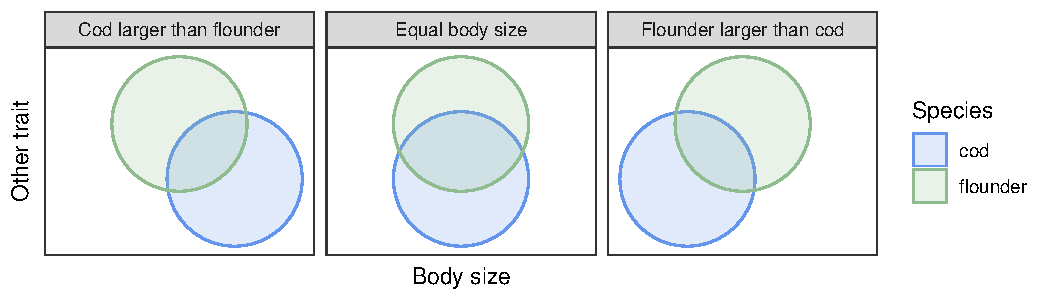
\includegraphics[width=0.95\textwidth]{fig-SI-overlap.pdf}
\caption{Illustration of possible trait distributions for cod and flounder in a two-dimensional trait space. The abscissa measures body size; the ordinate some other trait such as coloration, swimming speed, or preferred water depth. The circles show the 95\% contour lines of the bivariate normal trait distributions for cod (blue) and flounder (green). In the left panel, cod are larger on average than flounder; in the right, flounder are larger on average; and in the center, the mean body sizes are exactly equal. Despite their equality, the distributions do not fully overlap, beause of the difference in the other trait that is not under evolutionary influence. As a result, the trait overlap (and thus competition for shared resources) may remain partial even if the marginal distributions for body size match perfectly.}
\label{fig:overlap}
\end{figure}


\begin{figure}
\centering
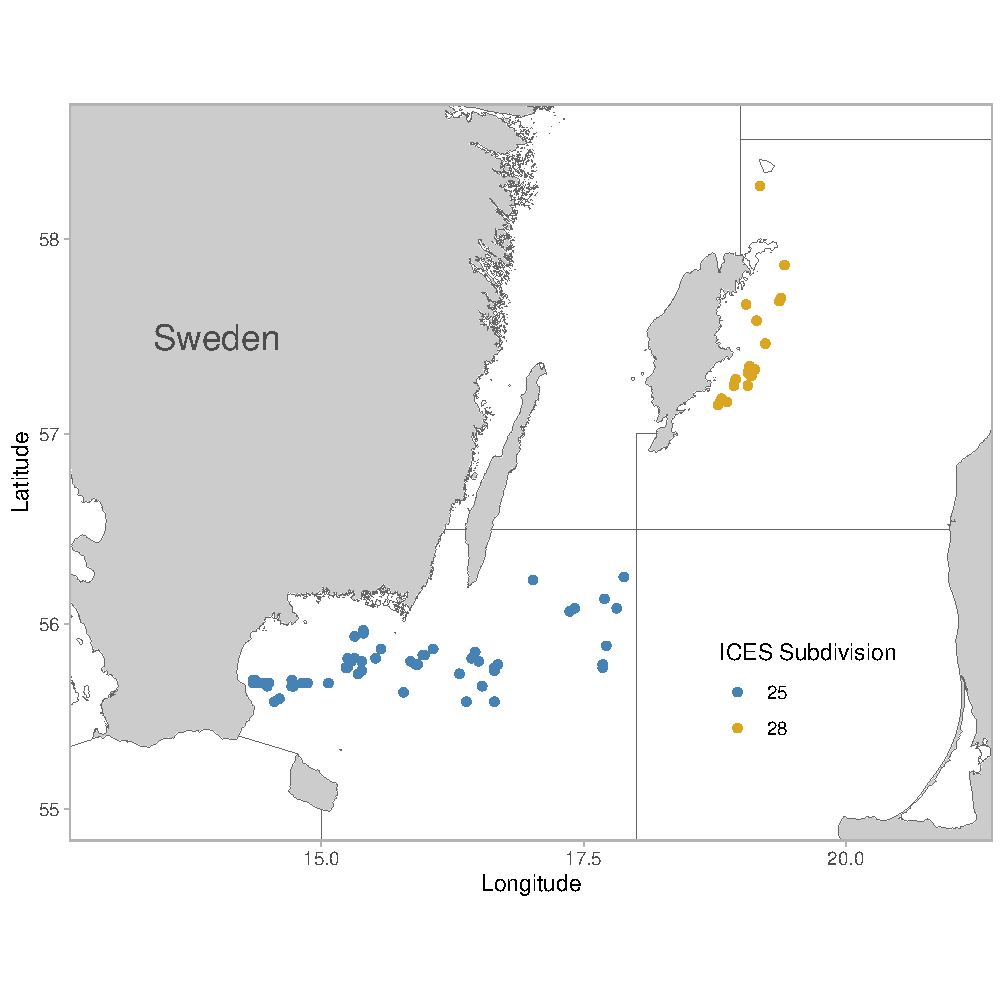
\includegraphics[width=0.8\textwidth]{figs1.pdf}
\caption{Catch locations of stomach content data from the Baltic International Trawl Survey (BITS) for years 2016-2018 and 2020.}
\label{fig:si_map}
\end{figure}

\begin{figure}
    \centering
    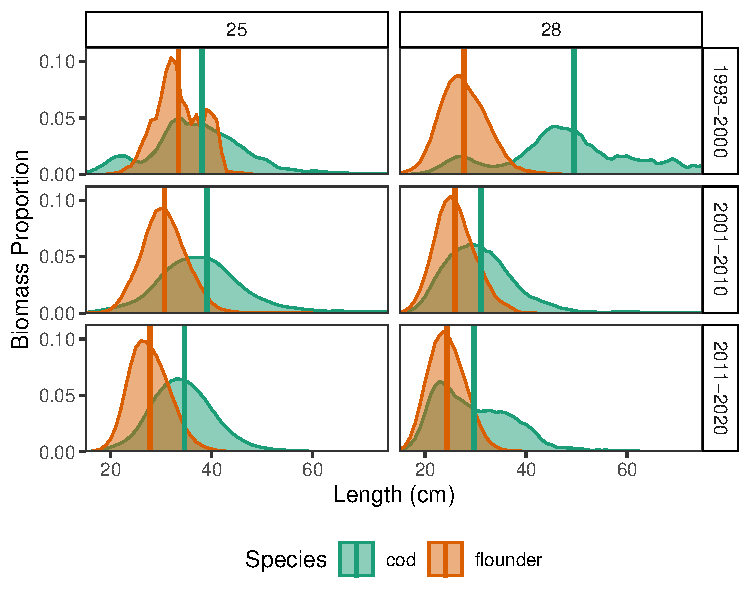
\includegraphics[width=0.7\textwidth]{figs2.pdf}
    \caption{Cod and flounder length distributions in ICES subdivisions 25 and 28. Data is aggregated to years listed in the facets for quarter 1 data. Vertical lines indicate mean length. Proportion is derived from the density of biomass for the specific lengths using 3 cm moving averages.}
    \label{fig:si_sizegrid_q1}
\end{figure}

\begin{figure}
    \centering
    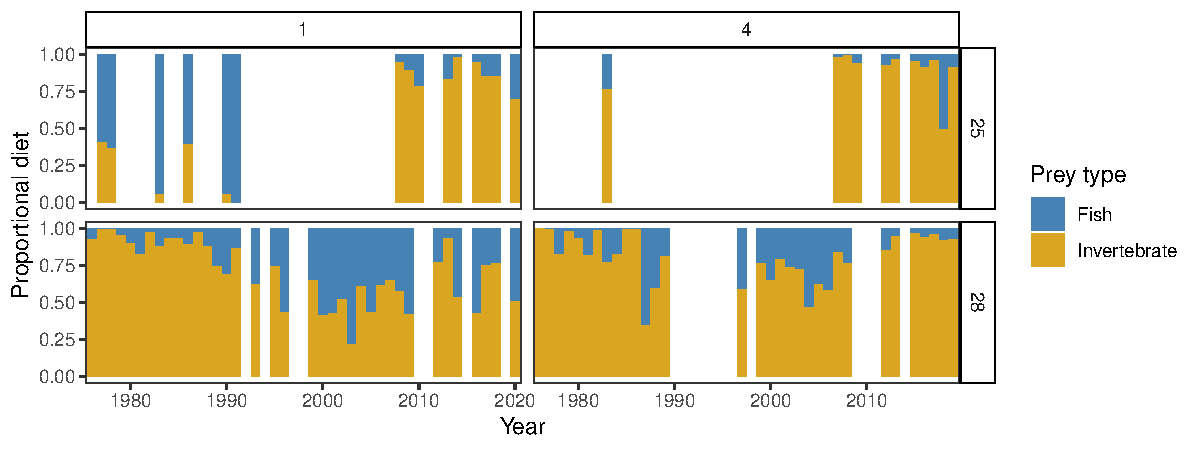
\includegraphics[width=1.0\textwidth]{figs3.pdf}
    \caption{Proportion of fish vs benthic invertebrate diet based on cod stomach content data for ICES subdivisions 25 and 28 in the Baltic sea. Data collected in quarter 1 and quarter 4 during years 1976-2020. Cod size for included individuals ranges 15-40 cm.}
    \label{fig:si_prop_fish}
\end{figure}

%%% Add this line AFTER all your figures and tables
\FloatBarrier


\bibliography{references}

\end{document}
